\section{Introduction}

Anomaly detection is an important tasks in several domains such as intrusion detection systems, financial fraud detection, especially in Internet of Thing (IoT). It has been estimated that collected data could contain from 2.3\% to 26.9\% error rate~\cite{goldberg2008analysis}. Applications built upon imprecise time series can potentially result in losses in the millions of dollars to businesses~\cite{cleaningSource}. As a concrete example, in forest fire detection many sensors are deployed to monitor the concentration of carbon-monoxide and various organic compounds \cite{alkhatib2014review}. Potential problems are detected before occurring by combining collected data with the external weather information (e.g., wind speed, temperature, humidity). Imprecise detection coming from abnormal data could significantly decrease the system reliability and results for remedial works. The efficacy of such system need to be in collusion with anomaly detection algorithms \cite{mehrotra2017anomaly}.\\

\par Anomaly detection over time series is often applied to filter out dirty data. This means that the detected points are discarded as useless noises. Unfortunately, the eliminated data may contain notable events, also known as {\em change points}. These changes occur by accident (e.g., a fire in a forest) or because of human intervention (e.g., watering the tree). Preserving these events is essential to interpret the context. For example, to optimize the watering schedule, a city environment management company deploys the sensors to monitor the impact of watering on soil humility under the trees. However, a significant increase of soil humility due to water can be detected as anomaly and removed from the data~\cite{kang2013prevention}. Thus, the ability to explicitly distinguish between anomalies and events is needed.\\

\par The first plot from the top in Figure~\ref{fig: picture 1} visually presents this challenge in real ultrasonic sensor data that we obtained from an IoT solution company. The sensor is plugged on the top of a tank to monitor its liquid level (y axis) over time (x axis). As shown in the figure, some sudden changes appear, either in isolation (time index 100, 140) or as small groups (time index 230). These are likely the abnormal values, such as sensor errors, and should be fixed or removed from the data set. On the other hand, the data change generated by filling the tanks (time index 280) should be preserved.\\

\par The most common anomaly detection methods on time series use traditional statistical methods, e.g., neighbor-based \cite{chandola2009anomaly}\cite{Breunig:2000:LID:335191.335388}\cite{tang2001robust}\cite{kriegel2009loop}, ensembles \cite{skyline}\cite{Pevny2016} or probabilistic models \cite{burnaev2016conformalized}\cite{ahmad2017unsupervised}. They consider a data point as an abnormal if it significantly differs from historical observations. Unfortunately, change points also have this property in practice. The detection methods recognize such change points as anomaly. For state-of-the-art anomaly detection methods such as Numenta\cite{ahmad2017unsupervised}, KNN-CAD\cite{burnaev2016conformalized}, the presence of change points in times series significantly decrease the quality of detection. This often leads to skip other true anomalies. The basic idea of Numenta and KNN-CAD is to use a training set ($x_1, …., x_m$) from historical data to predict the value of $x_{m+1}$. Then, they compute a measure of prediction error. At final step, the use a probabilistic model to estimate the anomalous state. The presence of change point in the historical data will directly affect the prediction result by disordering the sequence in training set. If these algorithms predict an abnormal point as a change point. This point could be ignored because the prediction error is minor. As shown in Figure \ref{fig: picture 1}, Numenta algorithm ignores all collective anomalies. The KNN-CAD fails in all its detection.
In addition, the performance of such detection highly depends on parameter configuration data specific. Owing these limitations, the detection result is very poor (The f-score is under 20\%), as illustrated in both Figure \ref{fig: picture 1} in problem statement and empirical experiments in the evaluation section.\\

% \paolo{explain that only part of the data is in the figure}

\par Since completely automatic anomaly detection might not work well without discrimination between anomalies and change points. One approach is to use supervised learning method \cite{agrawal2015survey}\cite{gonbadi2015supervised}\cite{ma2016supervised}. However, labeled data is not available in general. This motivates our idea to exploit on interactive approach. The goal is to minimize the user involvement while guaranty quality over the results of the process. This is achieved by an  active learning method is exploited to obtain the truth from users. Our experiments show that labeling a very limited number of data points can significantly increase the detection quality. 
To reduce the number of interaction, we propose a non-parametric algorithm, which accurately detects both anomalies and change points based on the combination of a novel concept of neighborhood, namely {\em Inverse Nearest Neighbor} (INN) and unsupervised probabilistic classification. The philosophy of INN derives from observing objects in reality. Two objects have close-bond if they have a two way connection. Applying this concept to data object, object A and object B have strong relation if A is the neighbor of B and vice verse, B is the neighbor of A. More detail of INN is described in Section 2.4. Leveraging the advantages of INN, the type of a data point can be classified through evaluating as set of scores, that are calculated from INNs properties. The benefit of INN concept is also demonstrated in detecting collective anomalies. If a data point is identified as a abnormal points, its INNs is highly anomalous. Our algorithm will propagate the anomaly score to such INN to expose the whole anomaly pattern. The Figure \ref{fig: innvsknn} illustrates the difference of INN and K-Nearest Neighbor (KNN). When evaluating a data point belongs a collective anomaly, its INN will be the entirety of such anomaly while its KNN contains both anomalous and normal points. We discuss more detail about novelties of INN in section 2.4.\\

\begin{figure}[ht]
	\centering
	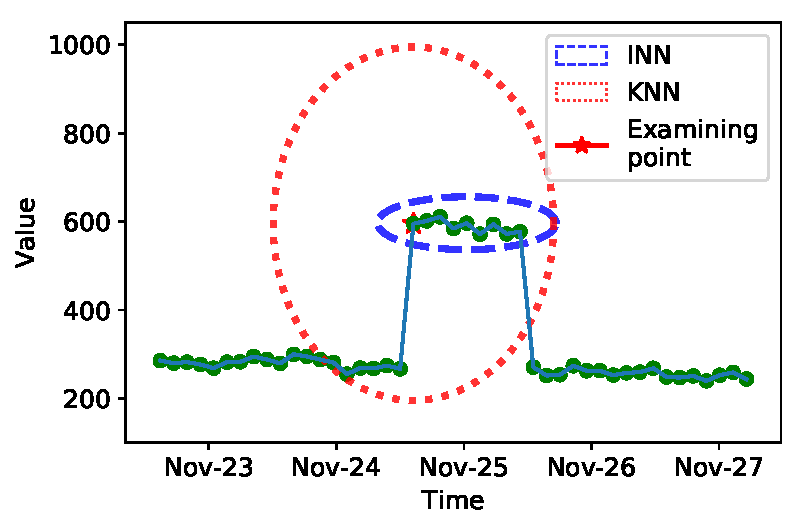
\includegraphics[width=0.8\textwidth]{Part3/Chapter7/figures/innvsknn.pdf}
	\caption{ : Compare Inverse Nearest Neighbor and K-Nearest Neighbor}
	\label{fig: innvsknn}
\end{figure}

\par Depending on the user-cases, user requires different detection quality. For example, fleet management application strongly requires high accuracy in discriminating the sensor errors and filling tank event while monitoring applications such as CO2 or temperature do not require such level of accuracy. This requirement leads to a new challenge how to satisfy user's desired quality why minimizing the user interaction? To address this challenge, the confidence of the classification model is used as termination condition for active learning process. More accuracy demands more points labeled to enrich the model until the classify confidence is achieved. Experiments demonstrate that with higher confidence requirement increases the F-score and it coverages to a consistent value.\\

\par Our method efficiently detects both anomalies and change points by taking advantages of Active Learning. We have implemented CABD as a python library. This prototype is empirically demonstrates producing high-quality detection in practical IoT user-cases. Our contributions in this work are summarized as follows:
\begin{itemize}
	\item CABD, a novel non-parametric algorithm for detecting both errors (i.e., single, collective anomaly) and events (i.e., breakpoints). 
	\item The novel concept of inverse nearest neighbor and active learning using uncertainty sampling scheme are applied to improve the CABD efficiency. 
	\item A prototype is implemented to evaluate CABD’s abilities in term of detection accuracy and response time in real IoT scenarios.
\end{itemize}
\par The remainder of this article is organized as follows. In Section 2, we formalize the problem of anomaly detection and related definitions. CABD is represented explicitly in Section 3. Section 4 evaluates quality of our method through two real use-cases. Section 6 discusses related works, and conclusion is presented in Section 7.  

\section{Preliminaries}
\subsection{Anomaly Types}

Anomaly detection is a technique used to identify unusual patterns that do not conform to expected behaviors, also called outliers. There are many applications in business, from intrusion detection to system monitoring. It is important to establish some boundaries on the definition of an anomaly. Anomalies can be broadly categorized as \cite{chandola2009anomaly}:
\begin{itemize}
	\item \textbf{Point anomalies}: A single instance of data is anomalous if it is significantly different from the remaining data.
	\item \textbf{Contextual anomalies:} The abnormality is context specific. This type of anomaly is common in time-series data. For example: 30 Celsius degree during summer is normal but may be abnormal in winter.
	\item \textbf{Collective anomalies:} This anomaly type contains a set of consecutive point anomalies to be represented as an abnormal data pattern. This pattern does not comply with the dataset distribution.
\end{itemize}

\subsection{Break Point}
In the simplest form, break point, also called change point, is the point at which the statistical properties of a sequence of observations change \cite{killick2014changepoint}. Break point detection is applied in vary application areas from finance, environment, health care to industrial maintenance~\cite{liu2013change}\cite{kawahara2009change}\cite{guralnik1999event}. More formally, let assume we have a time series $ X = \{x_1, x_2, ...., x_n\}$ which has $ m $ break points at the position $ \mathcal{C} = \{ c_1, c_2, ...., c_m \} $ with $ c_m < n $. The break points separate the data set into $ m + i $ segments such that the statistical properties of $ i^{th} $ segment $ \{ x_{c_{i-1}}, ... , x_{c_i} \} $ and $ (i+1)^{th} $ segment $ \{ x_{c_{i}}, ... , x_{c_{i+1}} \} $ are different in some way


\section{Problem Statement}
We consider a time series $ X = \{x_1, x_2, ...., x_n\}$ of $ n $ observations, where $ x_i $ is the $ i^{th} $ data point, may contain both errors and events. Its errors could be either single or collective anomalies and occur randomly. The main considerations are that, first, the event in X is usually detected as anomaly and simply discarded. Secondly, the detection performance is highly depends on configuration parameters which are data specific. Moreover, the present of change point also reduces such performance. Lastly, labeling anomaly data for training set requires immense manual labour. 
\par Let $ ac_i = \lbrace x_i, \ldots, x_{i+s} \mid x \in X, s \in \mathbb{N} \rbrace$, $as_i$ and $c_i$ denote a collective anomaly sized $ s $, single anomaly, change point at data point $x_i \in X$ respectively. The problem statements of our algorithm are formalized as follow:\\

\textbf{\textit{Problem:}} \textit{Given a desired detection quality and time series $ X = \{x_1, x_2, ...., x_n\}$, which has randomly abnormal points including both single and collective anomaly \\$ \mathcal{A} = \{ac_i, as_{t}, \ldots\}; $ $ i, t \leq n $ and a set of change points $ \mathcal{C} = \{ c_1, c_2, ...., c_m \} $ with $ m < n $. We aim to detect both $A$ and $C$ under a certain confidence level corresponding to the given quality while minimizing user interaction. 
}
\\
\par\textbf{Example 1} \textit{Consider time series X, a part of real IoT sensor data, has a collective anomaly occurring around Nov-24 and three single anomalies at Nov-10, Nov-14 and Nov-30 respectively. This time series also contains a change point about Dec-01. As shown in Figure~\ref{fig: picture 1}, all reviewed detection algorithms can not correctly detect the abnormality. For example, Numenta can not detect the sequence of errors and confuses change point with abnormal point. The detection result of KNN-CAD is even worth than Numenta. All single anomalies are mis-detected as collective anomalies. Our goals is to effectively detect both various kind of anomalies and change points in a single algorithm.}


\section{Inverse Nearest Neighbor}


\textbf{Definition 1}~(k-distance and nearest neighborhood of \textbf{p}): The k-distance of \textbf{p}, denoted as $ k_{dist}(p) $, is the distance $ d(p,o) $ between \textbf{p} and \textbf{o} in \textit{D}, such that for at least \textit{k} objects $ o' \in D/\{p\}  $ it holds that $ d(p,o') \leqslant d(p,o) $\\

\textbf{Definition 2}~(k-Nearest Neighborhood): The k-nearest neighborhood of p, denoted by $ NN_k(p) $ is the set of objects X in D with $ d(p,X) \leq k_{dist}(p) $.
\begin{equation}\label{key}
KNN_k(p)=\{ X \in D\/\{p\} | d(p,X) \leq k_{dist}(p) \}
\end{equation}

\textbf{Definition 3}~(Inverse Nearest Neighbor at k-distance): Given the time series $ X = \{x_1, x_2, .... , x_n\} $ and $x_i, x_j \in X$, if point $ x_i $ belongs to the nearest neighbor of point $ x_{j}$ at k-distance and vice versa, the point $ x_{j} $ belongs to the nearest neighbor of point $ x_{i} $ at k-distance, $ x_{j} $  is called as inverse neighbor of $ x_i $ at $k-distance $, denoted as:
\begin{equation}
\label{EQ: INN-definition}
 INN_k(x_i) = x_{j} \text{ \textit{iff} } 
 \begin{cases}
 x_i \in KNN_k(x_{j}) &     \\
 x_{j} \in KNN_k(x_i) & 
 \end{cases} 
\end{equation}

Inverse Nearest Neighbor at k-distance is the extended concept of Nearest Neighbor \cite{Huang2016} which lacks of checking reverse relation. The main purpose of INN is to identify the relation of two close data points. In reality,a data point and its INN may have the same characteristic. If this data point is anomalous, its INNs are highly anomalous which is in inverse proportion to their distance. That means the closer INNs have higher probability to be abnormal than others. The algorithm of finding INNs of a data point is described in Algorithm 1 that can automatically operate without any spacial parameters. In addition, we apply KD-tree~\cite{muja2009fast} to enhance searching performance.

\begin{table}[h]
	\centering
	\begin{tabular}{l}
		\toprule
		\textbf{Algorithm 1:} INN Searching of data point $ X_i $\\
		\midrule
		\textbf{Input: } kd-tree of time series X and data point $ X_i $ \\
		\textbf{Output:} List of INN's $ X_i $ \\
		1.~ Initializing: flag = 0, k = 1, $ INN(X_i) = \varnothing $	 \\
		2.~ Use kdtree to find the $ k $ nearest neighbors $ Y $ for $ X_i $ \\
		\hspace{10mm}$
		\left \|  
		\begin{tabular}{l}
		Find the $ k $ nearest neighbor for each $ Y_i \in Y $  \\
		\textbf{If} $ X_i \in KNN(Y_i)$ \textbf{and} $ Y_i \notin INN(X_i)  $ \textbf{then} \\
		\hspace{10mm} $ INN(X_i) = INN(X_i) \cup (Y_i,k) $  \\
		\end{tabular}
		\right .
		$\\
		3.~ Compute the size $ NNK(X_i) $\\
		\hspace{10mm} \textbf{If} this size does not changed \textbf{}\\
		\hspace{10mm} \hspace{10mm} \textbf{Return} $ NNK(X_i) $ \\
		\hspace{10mm} \textbf{Else}\\
		\hspace{10mm} \hspace{10mm} k++ \\
		\hspace{10mm} \hspace{10mm} go to step 2\\
		\hspace{10mm} \hspace{10mm}\\ 
	\end{tabular}
	\label{tab:INN_searching}
\end{table}
\begin{figure}[ht]
	\centering
	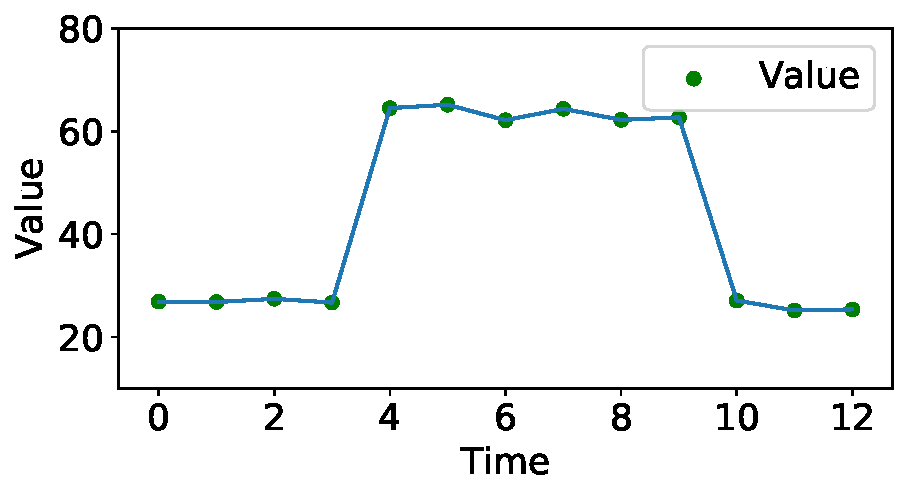
\includegraphics[width=0.8\textwidth]{Part3/Chapter7/figures/innvsknn_1.pdf}
	\caption{ : An Example of INN}
	\label{fig: innvsknn_1}
\end{figure}

\textbf{Example 2} \textit{\label{ex: 2} Consider the time series $X = $ \{26.87, 26.8, 27.42, 26.69, 64.51, 65.16, 62.15, 64.37, 62.21, 62.71, 27.07, 25.17, 25.364\} with thirteen data points in Figure~\ref{fig: innvsknn_1}, which contains collective anomaly on six points from $x_4$ to $x_9$. Assuming that we would like to find the INN of $x_4$. Let start at k = 1, we have $KNN_1(x_4) = \{x_5\}$ and $KNN_1(x_5) = \{x_4\}$. Referring to Equation~\ref{EQ: INN-definition}, $x_4$ and $x_5$ are INN at distance 1. Similarly, with k value from 2 to 5, we identify $\{x_6,\ldots,x_9\}$ belonging INN of $x_4$ \\
Let describe in detail at $k=6$, for simplicity, we use Euclidean Distance to calculate the distance between data points. With $
d(x_4, X) = $[37.86, 37.83, 37.14, 37.03, 0.0, 1.19, 3.09, 3.0, 4.61, 5.31, 37.93, 39.76, 39.96], we have $KNN_6(x_4) = \{x_5, \ldots, x_9, x_3\}$. Because of $\{x_5,\ldots,x_9\} \in INN(x_4)$, we will exam $x_3$. Using Euclidean Distance, we calculate $d(x_3, X) = $ [3.01, 2.0, 1.24, 0.0, 37.03, 38.52, 35.59, 37.89, 35.87, 36.52, 7.01, 8.14, 9.1]. Based on this distance we have $KNN_6(x_3) = \{x_0,x_1,x_2, x_{10}, x_{11}, x_{12}\}$. As we see, $x_3 \in KNN_6(x_4)$ but $x_4 \notin KNN_6(x_3)$. Therefore, $x_3$ does not belongs KNN of $x_4$. The INN searching for $x_4$ is stopped.}\\

\textbf{Definition 4}(Absolute first difference). The absolute value of first difference of $ x_{i} \in X $, denoted as $ \triangle x_i $, which is defined that:
\begin{equation}\label{First_difference}
\triangle x_i(p) = |x_{i}(p) - x_{i-1}(p)|,\, i = 1, 2, 3, ..., n
\end{equation}

\textbf{Definition 5}(Absolute Second difference). The absolute value of second difference of  $ x_{i}(p) $, denoted as $ \triangle '' x_i $, which is defined that:
\begin{equation}\label{Second_difference}
\triangle '' x_i(p) = |\triangle x_{i} - \triangle x_{i-1}|,\, i = 1, 2, 3, ..., n
\end{equation}

\textbf{Example 3} \textit{Consider again the time series in Example 2 $X = $ \{26.87, 26.8, 27.42, 26.69, 64.51, 65.16, 62.15, 64.37, 62.21, 62.71, 27.07, 25.17, 25.364 \}. Referring to Equation~\ref{First_difference}, the absolute first and second difference of $x_3$ are $\triangle x_3 = |x_3-x_2| = |27.42 - 26.8| = 0.62$ and $\triangle '' x_3 = |\triangle x_3 - \triangle x_2| = ||27.42 - 26.8| - |26.8 - 26.87| = 0.54|$}\\

\textbf{Definition 6}(Decay value). Decay value is the constant decrease in time. For example: $ x_i = 1 $, decay value = 0.2, so that $ x_{i+1} = x_i - decay \, value = 0.8 $

\section{Detection Algorithm using Active Learning}

Unlike the existing anomaly detections that only targets on detecting either single or collective anomaly and share common vulnerability to parameter configurations. We propose a comprehensive detection, being aware of both the anomaly and change point. In addition, applying Active Learning is not only significantly increase the accuracy but also reduce the sensitivity of (optimize) parameter configurations. In this section, we first present the overall algorithm. Then, we briefly explain each step along with related definitions.

\subsection{Overview algorithm}
Let $ X = \{x_1, x_2, ...., x_n \} $ denotes a time series, where Y and Z are set of anomaly points and break points of X respectively. Algorithm 2 presents the major steps of our proposal, which takes X as an input and produces Y and Z including their confident weights. Our algorithm also allows end-users to configure the desired confidence weight to ensure detection quality. The major steps are described as below:
\begin{enumerate}
	\item \textbf{Candidate Estimation}, in Line 1, generates the potential candidates, denoted by $ \theta $, from the extreme values in time series based on absolute second derivative.  
	\item \textbf{Score Computation}, in Line 3, computes score metric from INN of each candidate $ x_i $ in $ \theta $. This metric includes magnitude score, correlation score and variance score, denoted as $ \beta^{(x_i)} $
	\item \textbf{Score Evaluation}, in Line 4, uses a probabilistic classification to classify the candidates into three classes including change points, single anomaly points  or collective anomaly replied on the score metric. Active learning using the uncertainty model, described in equation \ref{equation:uncertainty_score}, is also applied. The most uncertain points will be queried and labeled to optimize the classifier. The output of this step is the confidence weight (CW) (denoted as $ \eth^{(x_i)} $) which is also known as anomaly score.
	\item \textbf{Anomaly Score Propagation}, propagates the anomaly score to its INNs in case the examining point is detected belonging to an anomaly pattern.
	\item \textbf{Classification Evaluation}, is the step to trigger the active learning process if the minimum of confidence weight is lower than user's quality requirement.

\end{enumerate}


\begin{table}[h]
	\centering
	\begin{tabular}{l}
		\toprule
		\textbf{Algorithm 2:} Anomaly and Change Point Detection\\
		\midrule
		\textbf{Input: } time series X, threshold $ \gamma $ (optional) \\
		\textbf{Output:} Error list $ Y $, change point list $ Z $ \\
		1.~ $ \theta \leftarrow $  Candidate(X) \\
		2.~ Y, Z = [ ] \\
		3.~ \textbf{For} $ x_i $ \textbf{in} $ \theta $ \textbf{do} \\
		\hspace{10mm}$
		%\left \|  
		\begin{tabular}{l}
		$ \beta^{(x_i)} \leftarrow $ Score($ x_i, X $) \\
		%$ \eth^{(x_i)} \leftarrow $ Evaluate($ \beta^{(x_i)} $)\\
		%$ UC^{(x_i)}, Y, Z \leftarrow $ Evaluate Detection($ \eth^{(x_i)} $)\\
		
		\end{tabular}
		%\right .
		$\\
		4.~  $ \eth^{} \leftarrow $ Evaluate($ \beta^{} $)\\
		5.~ $ CW^{}, Y, Z \leftarrow $ Evaluate Detection($ \eth^{} $)\\
		6.~  Y $\leftarrow$ Score Propagation($ \eth^{} $)\\
		7.~  \textbf{If} min(CW) $ \leq \gamma $  \textbf{then} \\
		\hspace{10mm}\textbf{Labeling} and \textbf{Go} to step 4 \\
		\\
		\hspace{5mm}\textbf{Return} $ Y, Z $\\
	\end{tabular}
\end{table}

\subsection{Anomaly Candidate Estimation}
Our goal is to intensively recognize both of errors and events. Therefore, we first introduce a method to identify the critical change in time series which also includes the detection of anomalous behavior. \\
Standard summary statistic such as mean, variance or correlation are common used in change detection. In our algorithm, we define the change of a point in time series based on its absolute second derivative. Formally, given time series X = {$ x_1, x_2,..., x_n $}. The change score of $ X $ is denoted by $ \partial $:
\begin{equation}\label{anomaly_score}
\partial(X) = \{\triangle"x_1, \triangle"x_2, ... ,\triangle"x_i\} | i \in \{1,2,...,n-1\}
\end{equation}
To identify the candidate, we use the statistically median absolute deviation (MAD) which is robust to anomalous data \cite{hochenbaum2017automatic}. If MAD of the change of a point is higher overall MAD standard deviation over the change of the whole data set, it is considered to be practically abnormal candidate. We will validate these candidates in the latter detection steps.\\
\par\textbf{Definition 17} Given time series X and the change score $ \partial $, MAD is defined as the median from sample median. 
\begin{equation}
MAD(X_i) = median(|\partial(X_i) - median(\partial(X))|)
\end{equation}

%Subsequently, we identify the peaks by using basic differentiation properties that the first derivative of a peak has a downward-going zero-crossing \footnote{\url{https://en.wikipedia.org/wiki/Zero_crossing}} at the peak maximum \cite{o1997pragmatic}. In the real-time series dataset, there are many false detections due to the noise. Therefore, the first derivate is smoothed before identifying downward-going zero-crossing. The extracted peaks are considered as the potential candidates for anomaly and change points. We will validate these candidates in the latter detection steps.\\
%\textit{Example:}....................\\

\subsection{Score Computation}

\par \textbf{Definition 7}(Spreading pattern) Spreading pattern (SP) of a data point is a set of data points from the examining point to its farthest INN. \\

\par \textbf{Definition 8}(Spreading size) Spreading size (SS) of a data point is the size of its SP. \\

\par \textbf{Definition 9}(Magnitude score) Magnitude score (MS) of data point is the radio of its Spreading Size over the size of dataset, denoted by MS. Given time series $ X = \{x_1, x_2, ..., x_n\} $ length $ n $ and $ x_i \in X $, the $ x_i $'s MS is defined as:
\begin{equation}\label{key}
MS(x_i) = \frac{SS(x_i)}{n}
\end{equation}

\par \textbf{Definition 10}(Piecewise Aggregate Approximation) Piecewise Aggregate Approximation (PAA) [*] transforms a time-series X of length n into vector $ \bar{X}=(\bar{x}_{1},.....,\bar{x}_{M}) $ with $ M \leq n $ where: \begin{equation}\label{PAA}
\bar{x}_{i} = \frac{M}{n} \sum_{j=n/M(i-1)+1}^{(n/M)i} x_{j}
\end{equation}

\par \textbf{Definition 11}(Symbolic Aggregate Approximation) Symbolic Aggregate Approximation (SAX) transforms a time-series X of length n into an arbitrary string by using PAA. A time series X length n can be represented by a word $ \hat{X} = \{\hat{x_1},\hat{x_2},....,\hat{x_n}\} $ with $ \hat{x_i} $ is a character of alphabet. Let denoted $ \alpha_j $ is the $ j^{th} $ element of the alphabet. $ \theta_{j-1} $, $ \theta_{j} $ are given thresholds.  
\begin{equation}\label{SAX}
\hat{x_i} = \alpha_j \,\,\,\,\,\, s.t \,\,\,\,\,\,\, \theta_{j-1} \leq PAA(x_i) \leq \theta_{j}
\end{equation}

\par \textbf{Definition 12}(Correlation Score) Correlation Score (CS) of a data point is the frequency of its Spreading pattern, which is represented as a string by using PAX. Given time series $ X = \{x_1,x_2,....,x_n\} $ and $ x_i \in X $
\begin{equation}\label{key}
CS(x_i) = frequency\left(\frac{SAX(SP(x_i)}{SAX(X)}\right) 
\end{equation}

\par \textbf{Definition 13}(Spreading pattern with k-neighbors) Spreading pattern with k-neighbors (SPk) of a data point is a set of data points from the point to its farthest INN including k adjacent points in both sides.\\

\par \textbf{Definition 14}(Variance Score) Variance Score (VS) describes the change of standard deviation of spreading pattern with k-neighbors after remove spreading pattern.
\begin{equation}\label{Variance Score}
VS(x_i) = \frac{std(X - INN(x_i))}{std(X)}
\end{equation}

As we discussed in previous section, the properties of a data point and its INNs are quite similar. Thus, we probably identify both point anomalies and collective anomalies through verifying its spreading pattern.
In this step, we compute the score metric of each candidate from step 1. There are three scores in this metric: (1) Magnitude score, (2) Correlation Score, (3) Variance Score. The detail of each score is clearly described in preliminary. In more detail, these scores are specifically represent the property of examining point. For example, magnitude score describes the proportion of spreading pattern of examining point in the dataset. Based on the anomaly definition, the size of anomaly  must be less five percent of dataset. Therefore, if the magnitude score is higher than five percent, the candidate probably is not an anomaly point. Similarly, correlation score represents the regularity of spreading pattern. \\

%Through these scores, we probably identify whether the candidates are abnormal points or change points. 
The algorithm 3 illustrates the score metric calculation process. We first find the farthest INN of examining point by using binary search which reduces significantly the complexity from $ n $ to $ log_2^n $. Next step, the scores are calculated in parallel to optimize performance. Finally, all score are collected and formed as a metric. 
\begin{table}[h]
	\centering
	\label{al-2}
	\begin{tabular}{l}
		\toprule
		\textbf{Algorithm 3:} Score Computation\\
		\midrule
		\textbf{Input: } Data point $ x_i $, time series X \\
		\textbf{Output:} Score Metric $ \beta^{(x_i)} $\\
		1.~ $ \eta \leftarrow $  SS($ x_i $, $ X $) \\
		2.~ $ \kappa \leftarrow $  MS($ x_i $, $ \eta $) \\
		3.~ $ \xi \leftarrow $  CS($ x_i $, $ \eta $) \\
		4.~ $ \varphi \leftarrow $  VS($ x_i $, $ \eta $) \\
		5.~ $ \beta^{(x_i)} \leftarrow $ [$ \kappa $, $ \xi $, $ \varphi $]  \\
		\textbf{Return} $ \beta^{(x_i)} $
		
	\end{tabular}
\end{table}

\subsection{Score Evaluation}

Replied on calculated metric scores, the Score Evaluation step uses a probabilistic classification algorithm to estimate the probability of data point $ x_i $ to be an anomaly point, change point or belonging to an anomaly pattern. CABD is designed with high modularity and flexibility. It allows to rapidly plug-play the classification algorithm depending on the context. By default, CABD use the random forest classification \cite{liaw2002classification}. Because of the variety of IoT scenario, obtaining a training set requires immense manual labour. Thus, without user intervention, the classification works on a set of initiated hypothesis. With the presence of human, the existing active learning using uncertainty sampling scheme \cite{cohn1994improving}, named CAL, is directly applied to increase classification performance by effectively labeling the most uncertain instances.\\ %The querying in CAL is made from the uncertainty of classification. \\

In CAL, we examine the most likely class of data points $ x_i \in X $ based upon the probability be done by classification algorithm. This probability is also considered as confidence weight of data instance. Then we decide whether or not to require its label $ y_i \in Y= $ \{abnormal point, anomaly pattern, change point\}  from human labeling process replied on the uncertainty of classification defined by:
\begin{equation}\label{equation:uncertainty_score}
\mathcal{U}(x) = 1 - P(\hat{x}|x)
\end{equation}
where $ x $ is the data point and $ \hat{x} $ is the most likely classification. The querying process of CAL is stopped if all confident weights are higher than a pre-configured threshold. By default, this threshold equals 0.8\\

\begin{figure}[h]
	\centering
	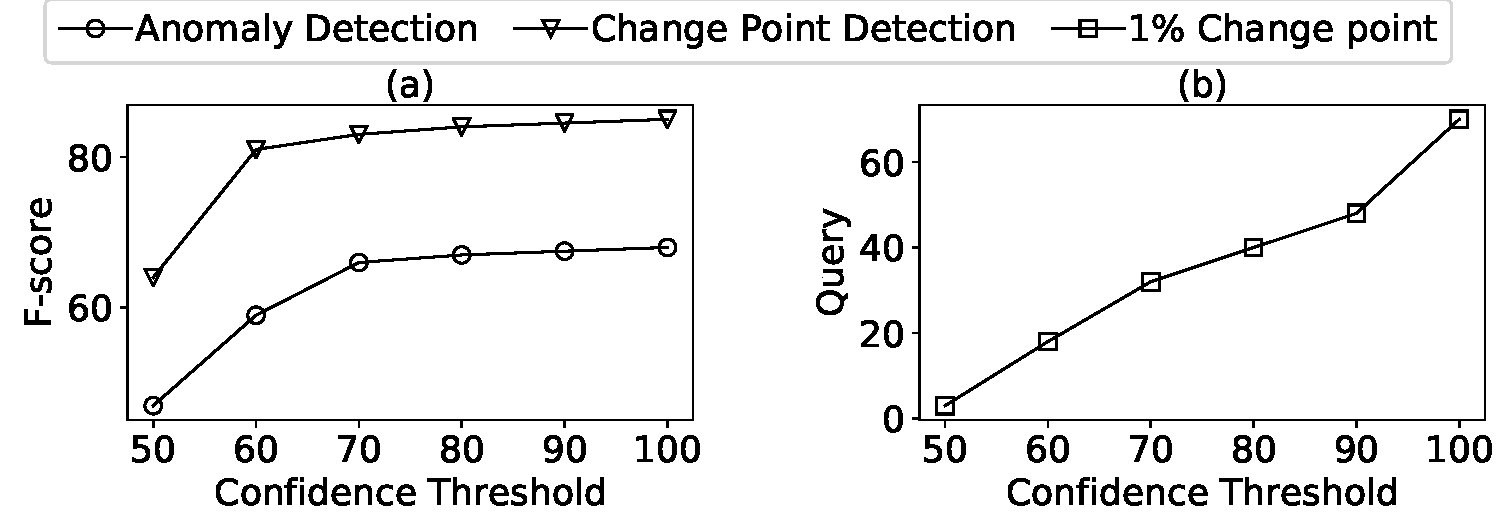
\includegraphics[width=\textwidth]{Part3/Chapter7/figures/new_compare_confidence.pdf}
	\caption{ : Varying confidence settings (a) Anomaly and Change point detection Accuracy, (b) The number of query}
	\label{fig:compare}
\end{figure}
\\
\textbf{Example } If data point $ x_i $ has classification possibility $ [0.1, 0.3, 0.6] $ to labels [abnormal point, anomaly pattern, change point], this point is the most likely change point with 0.6 confidence weight and $ 0.4 $ uncertainty. \\

The initial training set of the probabilistic classifier is build base on a set of hypothesis  $ \mathcal{H} $ which are include three main decision rules relied on score metric:

\begin{enumerate}
	\item The magnitude score (MS) of an abnormal point must be lower than $ k\% $. This means, the spreading pattern size of this point is lower than $ k\% $ of data size. Particularly, the spreading pattern size of single anomaly equals 1. 
	\item The correlation score of an abnormal point must be lower than $ c\% $. This means, the spreading pattern of this point must occur lower that $ c\% $ frequently in dataset
	\item The variance score of an abnormal point must be higher than $ v\% $. This means, the standard deviation of spreading pattern with k-neighbors must reduce at least $ v\% $ after removing the spreading pattern.
\end{enumerate}

From observing the properties of change point and various anomaly type in the practical dataset, we derive the set of threshold $ [k,c,v] $ is 0.05, 0.1 and 0.5 respectively. Given the set of examining data points X, label Y = \{abnormal point, collective anomaly, change point\}, threshold $ \theta =  [0.05, 0.1, 0.5]$, set hypotheses $ \mathcal{H} $ defined by:

\begin{equation}\label{hypothesis}
\left \{\begin{tabular}{c}
$ h_1 $ \, : \, \textbf{Anomaly Point} \quad \textrm{if} \quad $ \begin{tabular}{|l}
$ SS(x_1) = 1  $ \\
$ \beta^{x_i}_{\xi} \leq 0.1  $ \\
$ \beta^{x_i}_{\varphi} \geq 0.5  $ 
\end{tabular} $\\\\
$ h_2 $ \, : \, \textbf{Anomaly Pattern} \quad \textrm{if} \quad $ \begin{tabular}{|l}
$ \beta^{x_i}_{\kappa} \leq 0.05  $ \\
$ \beta^{x_i}_{\xi} \leq 0.1  $ \\
$ \beta^{x_i}_{\varphi} \geq 0.5  $ 
\end{tabular} $\\\\
$ h_3 $ \, : \, \textbf{Break Point} \quad \textrm{if} \quad $ \begin{tabular}{|l}
$ \beta^{x_i}_{\kappa} > 0.05  $ \\
$ \beta^{x_i}_{\xi} > 0.1  $ \\
$ \beta^{x_i}_{\varphi} < 0.5  $ 
\end{tabular} $\\
\end{tabular}
\right \}
\end{equation}


The algorithm 3 summaries the CAL for active learning in Score evaluation step. Let denote the $ \kappa $ and $ \varphi $ be the confident weight and uncertainty of data points respectively.

\begin{table}[h]
	\centering
	\label{tab:table2}
	\begin{tabular}{l}
		\toprule
		\textbf{Algorithm 3:} Score Evaluation\\
		\midrule
		\textbf{Input: } Unlabeled data set $ X $, probabilistic model $ Z $, \\ initial training set $ \mathcal{V} $, threshold $ \gamma $.\\
		\textbf{Output: } $ [\kappa $, $ \varphi $] \\
		1.~ [$ \kappa $, $ \varphi $] = Z(X,$ \mathcal{V} $) \\
		2.~ \textbf{While} $min(\kappa) \leq \gamma$ \textbf{do} \\
		\hspace{10mm}$
		\left \|  
		\begin{tabular}{l}
		$ x_t \leftarrow $ \textit{Query}($ x_t, \varphi ,X $) \\
		\textit{Label} $y_t$ for $x_t$\\
		\textit{Set} $ \mathcal{V} = \mathcal{V} \cup \{(x_t, y_t)\} $\\
		\textit{Update} $ [\kappa $, $ \varphi $] = Z(X,$ \mathcal{V} $)
		\end{tabular}
		\right .
		$\\
		
		
		\textbf{Return} $ [\kappa $, $ \varphi $]
		
	\end{tabular}
\end{table}

\subsection{Score Propagation}
The score propagation step selects the collective anomaly from the classification result and propagates the anomaly score to its INNs. The propagation step is control by decay values and the k-distance, this means the anomaly score of INNs near abnormal point to be more increased than others. By default, decay value of an data point equals the ratio of its anomaly score over its spreading size. Formally, given time series X, for each point $ x_i \in X $, $ \theta_{y_i} \in SP(x_i) $ is given by:
\begin{equation}\label{probagation_score}
\theta_{y_i} = \theta_{y_i} + \left( \theta_{x_i} - \alpha*k \right) 
\end{equation}
where $ \alpha = \frac{\theta_{x_i}}{SS(x_i)}$ and k are decay value and k-distance from $ x_i $ to $ y_i $ respectively. \\
\textbf{Example } Consider $ x_i $ has the anomaly score $ \theta_{x_i} = 0.8 $ and spreading pattern $ SP(x_i) = \left\lbrace [x_{i+1}, 1],[x_{i+2}, 2],[x_{i+3}, 3],[x_{i+4}, 4]\right\rbrace  $. The decay value of $ x_i $ is $ \alpha = \frac{0.8}{4} = 0.2$. Let assume $ \theta_{x_{i+3}} = 0.3 $, referring to Equation \ref{probagation_score}, we have anomaly score of $ x_{i+3} $ after propagating is:
\begin{equation*}
	\theta_{x_{i+3}} = 0.3 + \left( 0.8 - 0.2*3 \right) = 0.5 
\end{equation*}

\subsection{Complexity Optimization}
Among the major step in Algorithm, the Score calculation step is optimizable in searching INN of candidates. First, we identity that INN searching cost could be pruned by applying the binary search method which reduce the searching complexity from O(n) to O(Log n). Moreover, we add a new the stopping condition of INN searching based on maximum size of INN. \\

\textit{Intuition}: Recall that when searching the INN of data point x denoted INN(x) in Algorithm 1, the k value denoted the size if INN(x) starts at one and increases by one until k is not change. The complexity of such approach is O(k) with k is the size of INN(x). This could be optimized by using binary searching method to find the INN set for both side of examining point. The complete INN is the union of these sets. The complexity will be reduced from O(n) to 2*O(Log n). The operation of binary search requires maximum searching positions as an mandatory input. In practice, if the size of an abnormal pattern is higher than five percentage of data set, it could not be considered as collective anomaly. Thus this boundary is used as the maximum searching range.\\

Given data point $x_i$, searching range threshold $t$. The algorithm 4 illustrates the Binary INN searching for the right side of data point $x_i$
 
\begin{table}[h]
	\centering
	\begin{tabular}{l}
		\toprule
		\textbf{Algorithm 4:} Binary INN searching\\
		\midrule
		\textbf{Input: } Data point $x_i$, threshold t \\
		\textbf{Output:}  $INN_R(x_i)$\\
		1.~ $ L = i; R = t - 1; INN_R(x_i) = [ ]; $\\
		2.~ \textbf{While} $ L \leq R $ \textbf{do} \\
		\hspace{10mm}$
		\left \|  
		\begin{tabular}{l}
		$m = floor((L+R)/2)$ \\
		\textbf{If} $x_m \in KNN(x_i)$ \textbf{and} $x_i \in KNN(x_m)$\\
		\hspace{5mm}$ L = m + 1$\\
		\textbf{Else}\\
		\hspace{5mm}$ R = m - 1$\\
		
		\end{tabular}
		\right .
		$\\
		4.~  $INN_R(x_i) = [x_i, \ldots, x_m]$\\
		5.~  \textbf{Return} $ INN_R(x_i) $
	\end{tabular}
\end{table}


\section{Evaluation}


In this section, we experimentally evaluate the quality and efficiency of our proposal on both real and synthetic datasets. Such results are also compared with one of common anomaly detection approaches. Our goal is to demonstrate that:
\begin{itemize}
    \item The superiority of CABD in both detection quality (anomaly, change point detection) and runtime over real and synthetic datasets. 
    \item The effectiveness of INN concept and active learning in our propose.
    \item CABD could be a complementary part to enhance data repairing algorithms.
\end{itemize}


%In this section, we empirically evaluate the quality and efficiency of our proposal on both real and synthetic dataset. We demonstrate that:
%\begin{itemize}
%	\item CABD effectively detect both single and collective anomalies which need to be removed.
%	\item CABD quickly identify the key deviation event which also known as break point.  
%	\item Applying active learning significantly improves the CABD’s accuracy. 
%\end{itemize}
%We briefly describe each of these goals below

%\subsection{User studies}
%\subsubsection{User study 1: Tank Monitoring}
%\subsubsection{User study 2: Humility Monitoring}


\subsection{Metric of measurement}
For evaluating the efficiency of proposed algorithm, we use three common metrics named Precision, Recall and F-score. .Let S be the number of the outliers or change points detected by the algorithm and G be their ground truth. The precision (P) and recall (R) are defined as
\begin{equation}\label{Precision}
Presicion = \frac{|{S}|\cap{G}}{|{S}|}
\end{equation}
and
\begin{equation}\label{Recall}
Recall = \frac{|{S}|\cap{G}}{|{G}|}
\end{equation}
respectively. F-score or F-measure, a simple way to balance the P and R of an overall detection result, is defined as: 
\begin{equation}\label{F-score}
F\-score = 2 * \frac{P * R}{P + G}
\end{equation}

To assess the advantage of using interactive learning in comparison to manual update of all cases, we use a benefit function calculated from the cost ratio as the number of actions divided by the number of errors \cite{he2016interactive}. Formally, given the number of query by active learning $ T_A $ and manually update $ M $, we defined the benefit of the algorithm as: 

\begin{equation}\label{func: benefit_function}
BNF = 1 - \frac{T_A}{M}
\end{equation}

\subsection{Benchmark dataset}
\subsubsection{Real dataset}

\begin{figure*}[h]
	\centering
	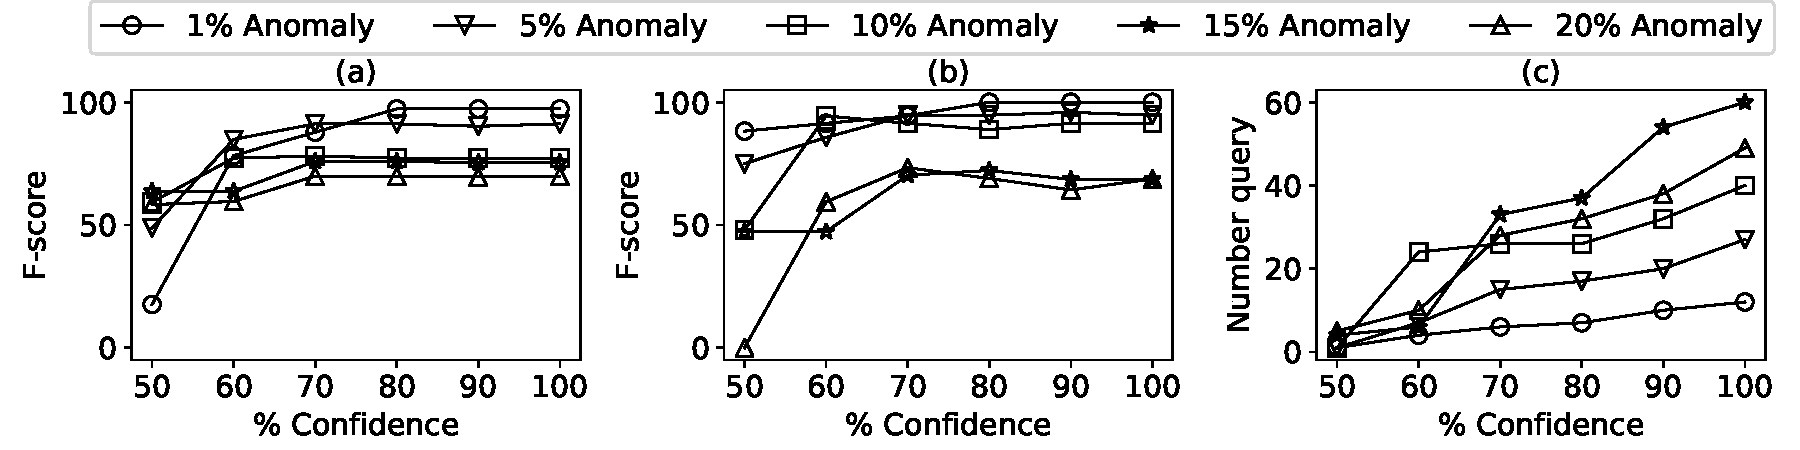
\includegraphics[width=\textwidth,height=\textheight,keepaspectratio]{Part3/Chapter7/figures/new_changeALpercentage_with1CP.pdf}
	\caption{ : Evaluation on varying Confidence Weight. From left to right, the three plots show: (a) Anomaly detection quality, (b) Change point detection quality, (c) The number of query to achieve given Confidence Weight}
	\label{fig: confident_1CP_compare}
\end{figure*}

\textit{IoT data with real errors:} The data is collected from 2 real ultrasonic sensors deployed on the top of tanks. Errors naturally occur without any human interactions ($ https://github.com/kimhungGCZ/anomaly\_dataset $) . Since we entirely manage the tank operations such as filling or consuming, the errors and change points are manually labeled as ground truth. \\

\textit{Yahoo data with real error:} The yahoo lab data ($ http://labs.yahoo.com/Academic\_Relations $) provides a number of datasets taken from real production traffic to some of Yahoo's properties. The abnormal points of such datasets are marked by humans so they are probably not consistent. In addition, the change points are not presented. Therefore, the datasets are best used to measure the recall factor of anomaly detection.

\subsubsection{Synthetic dataset}
Synthetic datasets aim to assess the efficacy of our algorithm in the presence of various anomaly types (local, global, single, collective anomalies) and change points in different proportion. To create these datasets, we first generate the data points following real data distribution. Then we fit this curve to a time series obtained from IoT production environment to preserve the trend and seasonality. Lastly, we randomly inject a mix of anomaly types with varying widths and magnitudes. These anomalies also recorded to evaluate against the points detected by our proposed algorithm. Figure \ref{fig: data_1_ex} illustrates a part of synthetic dataset named \textit{ds-1} that includes global, local and collective anomalies. Two notable events are also reported as the change points. 

\begin{figure}[H]
	\centering
	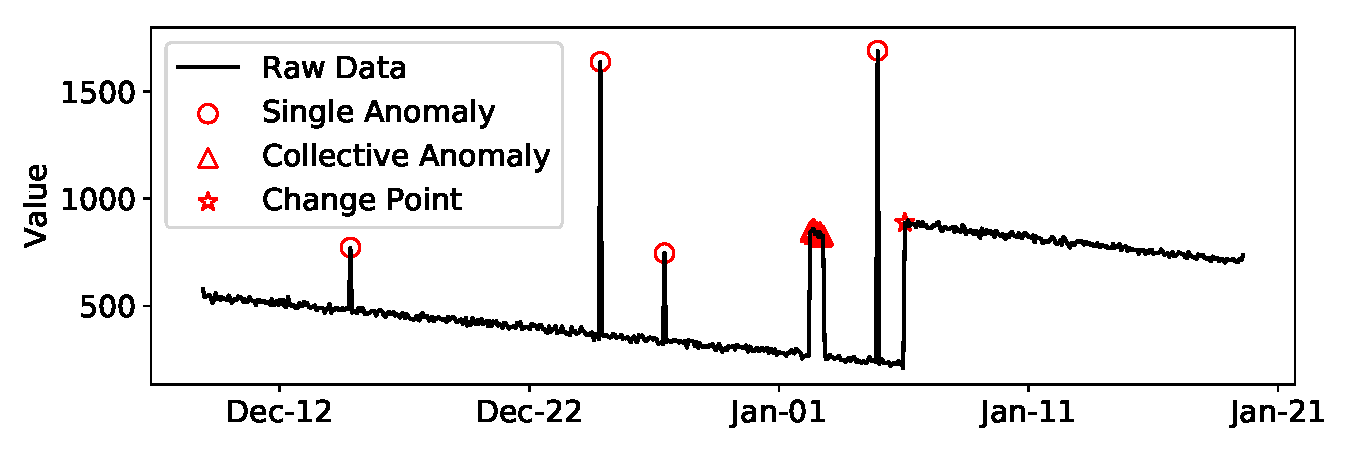
\includegraphics[width=0.8\textwidth]{Part3/Chapter7/figures/data_1_ex.pdf}
	\caption{ : An example of Synthetic dataset.}
	\label{fig: data_1_ex}
\end{figure}

\subsection{Results}
\subsubsection{Experiments on Real Errors}

We evaluate the detection quality our proposal over the real data sets provided by Yahoo and an IoT solution company. Since Yahoo does not record the change points, we only perform anomaly detection on such datasets. Table~\ref{tab:yahoo_data} reports Precision, Recall, F-measure and the number of query to achieve 80\% confidence weight over 50 Yahoo's datasets.\\

We present the notable results in the first part of this table. It is not surprising that Active learning significantly increases CABD's detection quality. Without active learning process, the average precision and recall scores were about 72.7\% and 77.2\% respectively. In some datasets, F-score achieved 100\% on average such as \textit{real\_3} and \textit{real\_6}, meaning that all detected points are totally correct without false. After applying active learning to optimize the probabilistic model, both the precision and recall score were converging to perfect value. The achieve results increased to about 96.8\% and 97.8\% for precision and recall values, respectively. Moreover, the query is very effective shown through low benefit score (0.5 on average). This means labeling a candidate could reveal 2 other abnormal points. \\

In further analysis, we analyze the worst results which are presented in the second part of Table~\ref{tab:yahoo_data}. Intensively investigating into such results, we realize that the false negatives usually occurs at the boundaries of abnormal data, especially at the ends of collective anomalies. \\

From two real IoT datasets shown at the end of Table~\ref{tab:gcz_data_synthetic}, we note that the anomaly detection's recall on average was 100\% without labeling requirement, this means all abnormal points are recognized. However, the overall F-scores of anomaly and change point detection only achieve about 57.3\% and 33.3\% respectively. Based on active learning, the F-score coverages to perfection at 100\% after labeling 1 candidate. These results prove again that our proposal is capable of effectively detecting both anomalies and change points with very few label requirement. %and coverage to high accuracy.
\\

\begin{table}[h]
\small
  \centering
   \small{
   \resizebox{\columnwidth}{!}{%
       \setlength\tabcolsep{2pt}
        \begin{tabular}{c|c|c|c|c|c|c|c}
        \multirow{3}[3]{*}{\textbf{Dataset}} & \multirow{3}[3]{*}{\textbf{\%AD}} & \multicolumn{1}{c|}{\multirow{3}[3]{*}{\textbf{\%CP}}} & \multicolumn{2}{c|}{\textbf{W/O AL}} & \multicolumn{2}{c|}{\textbf{W/ AL}} & \multicolumn{1}{c}{\multirow{3}[3]{*}{\textbf{\makecell{Total\\query}}}} \\
    \cmidrule{4-7}          &       &       & \multicolumn{1}{c|}{\multirow{2}[2]{*}{\textbf{\makecell{AP\\F-score}}}} & \multicolumn{1}{c|}{\multirow{2}[2]{*}{\textbf{\makecell{CP\\F-score}}}} & \multicolumn{1}{c|}{\multirow{2}[2]{*}{\textbf{\makecell{AD\\F-score}}}} & \multicolumn{1}{c|}{\multirow{2}[2]{*}{\textbf{\makecell{CP\\F-score}}}} &  \\
              &       &       &       &       &       &       &  \\
        \midrule
        Synthetic & 12.5  & 9.5   & 38.0  & 39.3  & 67.9  & 83.6  & 38.7 \\
        \midrule
        Yahoo & 1.0   & -     & 44.4  & -      & 80.0  & -     & 5.0 \\
        \midrule
        IoT & 0.8   & 1.0   & 53.7  & 33.3  & 100.0 & 100.0 & 4.0 \\
        \end{tabular}%
        }
      \label{tab:all_evaluation_results}%
       \caption{: Evaluating Anomaly Detection (AD) and Change Point Detection (CP) qualities on Synthetic, Yahoo and IoT datasets.}
       }
\end{table}%


\subsubsection{Experiments on Synthetic Errors}

Next, we evaluate CABD on the synthetic datasets which simulate various anomaly types and change points as real scenarios. Similar to real datasets, the detection qualities (both anomaly and change point detection) are measured in two phases: before and after executing active learning. Table \ref{tab:gcz_data_synthetic} presents the experiment results of varying anomaly and change point proportion. From this table we note that:\\

First, CABD with active learning significantly improves the detection accuracy. The average F-score increases from 38\% to 67.9\% and from 39.3\% to 83.6\% for anomaly and change point detection respectively. Remarkably, the active learning takes more advantage at low anomaly percentage. For example: in dataset with 1\% anomaly such as \textit{ds-1}, the F-score increase by about 80\% from 17.3\% to 97.3\% after learning. Similar results are also found in \textit{ds-6} and \textit{ds-11} datasets. \\

Second, the query selection of active learning is highly effective. The benefit score is about 0.88 on average, that means labeling 12 candidates could recognize 100 abnormal points. As shown in Figure~\ref{fig:comapration_benifit}, regardless the changes in percentage of anomaly and change point, the query benefit is consistent from 0.8 to 0.96. This result demonstrates that the model inputs (score metrics) calculated from Inverse Nearest Neighbor concept are highly related in detecting anomaly and change points. \\

Lastly, as illustrated in Figure~\ref{fig:comapration_AC}, high percentage of anomalies and change points could decrease the efficiency of CABD. In more detail, increasing the anomaly percentage from 1\% to 20\% will decrease the F-score by 27.4\% and 31\% for anomaly and change point detection, respectively. This can be explained that if a single anomaly point is very close to a change point, its spreading pattern based on inverse nearest neighbor will be larger than usual. Thus, the metric score of such point is very likely to a change point. This leads the classification model to conflict when labeling this point as a single anomaly. 

\begin{figure}[h]
	\centering
	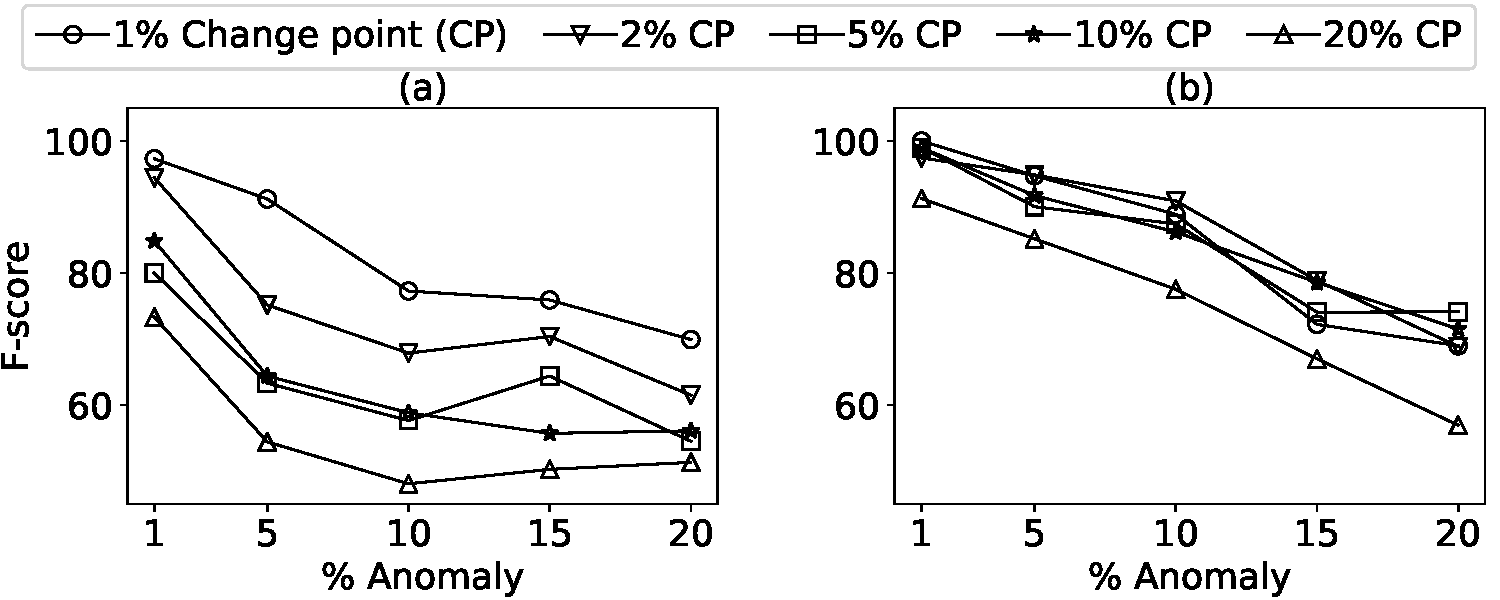
\includegraphics[width=0.8\textwidth]{Part3/Chapter7/figures/new_changeALpercentage.pdf}
	\caption{ : Varying the percentages of anomaly and change point over Synthetic data. From left to right, the two plots show:  (a) Anomaly detection quality, (b) Change point detection quality.}
	\label{fig:comapration_AC}
\end{figure}

\subsubsection{Runtime}
We experimentally compare the runtime of CABD and reviewed algorithms on various data sizes. All evaluations are performed on a computer with following configuration: Intel i5-6200U CPU @ 2.30GHz, 2 Core(s), 4 Logical Processor(s), 8GB of RAM and the operating system is 64-bit Windows 10. Since CABD is an active learning algorithm, labeling time of the end-user is not included. As shown in Figure~\ref{fig:comapration_timerunning}, the runtime of CABD roughly equals that of LOF and is extremely tiny comparing with Numenta or KNN-CAD at all data sizes. More details, with 2000 data points, Numenta and KNN-CAD process in 24.91 and 11.61 seconds, respectively, while the runtime of CABD is only around 0.16 seconds. The similar results are also found in the larger datasets. Numenta and KNN-CAD need 356.03 and 113.02 seconds respectively to detect the anomalies in 20000 data points whereas CABD needs 2.56 seconds. In summary, CABD could provide significant better in both detection quality and running time over the state-of-the-art algorithms.

\begin{figure}[h]
	\centering
	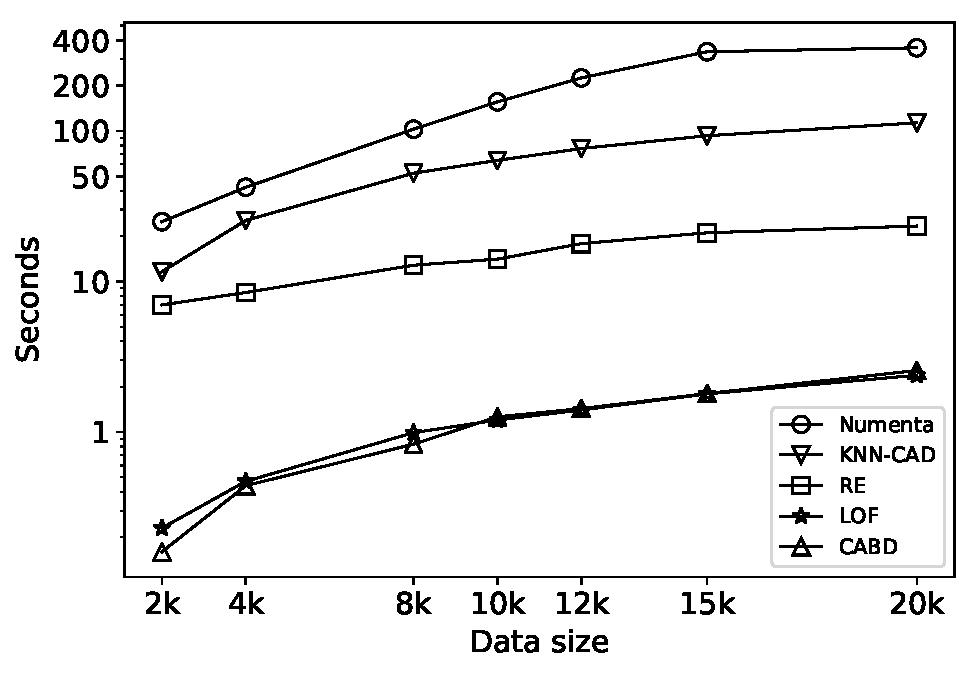
\includegraphics[width=0.6\textwidth]{Part3/Chapter7/figures/time_running_evaluation.pdf}
	\caption{ : Evaluating runtime of common Anomaly Detection Algorithms over different data sizes for Yahoo datasets.}
	\label{fig:comapration_timerunning}
\end{figure}

\subsection{Effectiveness of Active learning}

In our proposal, the Active learning process is an important step to achieve non-parametric algorithm and high accuracy in wide range user-cases. Summarizing evaluation results from Table~\ref{tab:gcz_data_synthetic} and \ref{tab:yahoo_data}, the detection quality of CABD with active learning always outperforms one of non-active learning. For example, the average f-score of anomaly detection on Yahoo datasets increases by 35.3\% from 61.8\% to 97.1\%. This stems from the fact that active learning could optimize the probabilistic classification model to be more accurate. \\

Table~\ref{tab:AL_queryrounds} presents the accuracy score (acc), minimum confident (cof) of the model in each round. The number of correct points (noc) detected from candidate list, which is done in Candidate Estimation step, also reported. From this table, we note that the model may identify all abnormal points (reach 100\% accuracy score) after a few queries.  For example, after 4 queries, the model in $ real\_1 $ dataset reaches 100\% accuracy with 21 data points be distinguished. In some round, the model accuracy decreases after labeling a candidate point. This can be described to the following: in case the abnormal point appears very close a change point pattern, the metric score of this point tends to similar with change point such as high magnitude score, correlation score, and low variance score. Thus, CABD detects the point as a change point. Consequently, labeling this point as an abnormal point will conflict with current mode awareness which leads to decrease mode accuracy. 

\begin{table}[ht]
  \centering
  \small{
        \setlength\tabcolsep{3pt}
        \begin{tabular}{|c|c|c|c|c|c|c|c|c|c|c|}
        \toprule
        \multirow{2}[4]{*}{\textbf{Round}} & \multicolumn{2}{c|}{\textbf{real\_1}} & \multicolumn{2}{c|}{\textbf{real\_23}} & \multicolumn{2}{c|}{\textbf{real\_42}} & \multicolumn{2}{c|}{\textbf{real\_iot\_1}} & \multicolumn{2}{c|}{\textbf{real\_iot\_2}} \\
    \cmidrule{2-11}          & acc   & conf  & acc   & conf  & acc   & conf  & acc   & conf  & acc   & conf \\
        \midrule
        1     & 0.1   & 0.5   & 0.0   & 0.5   & 0.0   & 0.7   & 0.8   & 0.7   & 0.9   & 0.7 \\
        \midrule
        2     & 0.1   & 0.4   & 0.6   & 0.5   & 0.1   & 0.5   & 1.0   & 0.6   & 1.0   & 0.7 \\
        \midrule
        3     & 0.6   & 0.4   & 0.5   & 0.5   & 0.2   & 0.5   & 1.0   & 0.7   & 1.0   & 0.7 \\
        \midrule
        4     & 0.6   & 0.4   & 0.7   & 0.7   & 0.6   & 0.5   & 1.0   & 0.8   & 1.0   & 1.0 \\
        \midrule
        5     & 1.0   & 0.6   & 0.8   & 0.6   & 0.4   & 0.4   &       &       &       &  \\
        \midrule
        6     & 1.0   & 0.6   & 0.8   & 0.5   & 1.0   & 0.6   &       &       &       &  \\
        \midrule
        7     & 1.0   & 0.8   & 1.0   & 0.7   & 1.0   & 0.4   &       &       &       &  \\
        \midrule
        8     &       &       & 1.0   & 0.8   & 1.0   & 0.9   &       &       &       &  \\
        \bottomrule
        \end{tabular}%
      \caption{: Active learning query round}
	\label{tab:AL_queryrounds}%
  }
\end{table}%

%\begin{figure}[h]
%	\centering
%	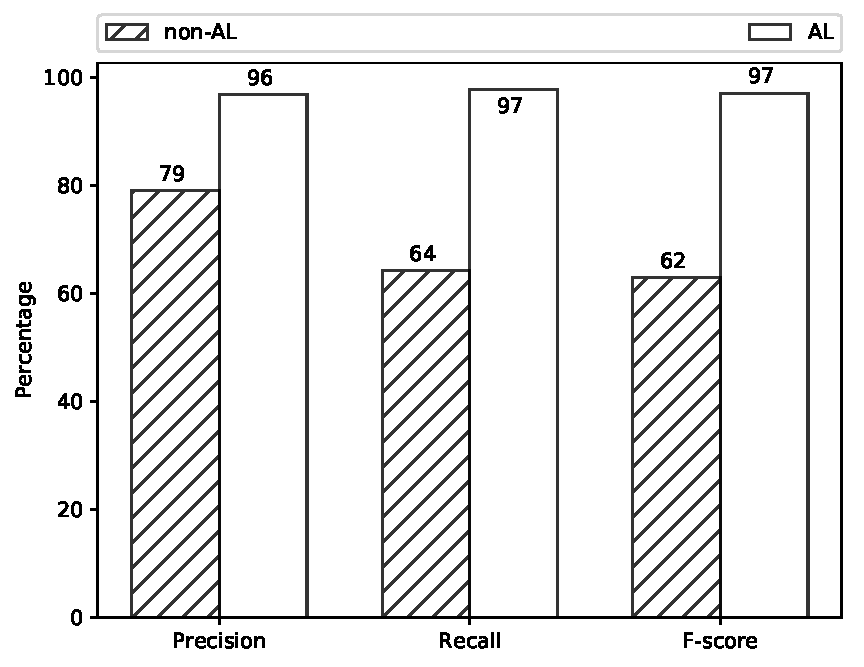
\includegraphics[width=0.5\textwidth]{comparation_percentage.pdf}
%	\caption{ : Comparison the F-score between CABD with and without active learning.}
%	\label{fig:comapration_percentage}
%\end{figure}




\subsection{Effectiveness of INN} 
\par Similarly active learning, Inverse Nearest Neighbor is a novel concept accelerating detection accuracy. Moreover, searching INN is a non-parametric algorithm. This makes INN robust to the sensibility of parameter configurations that is one of common limitations in reviewed algorithms. To demonstrate the efficacy of INN in comparison with KNN, we replace INN by KNN in our evaluation. The appropriate K parameter is determined by bruce-foced searching in range from 0 to data size. Such replacement is evaluated on both real and synthetic data sets. \\

As shown in Figure~\ref{fig:comapration_INNvsKNN_yahoo}, CABD using INN~(CABD-INN) shows better performance in comparison with one using KNN~(CABD-KNN) in both cases (with and without active learning). In details, the f-scores of CABD-KNN are reported around $31\%$ and $48.32\%$ for before and after active learning respectively. Replacing KNN by INN, the f-score significantly increases by 31.68\% to 80\% in case performing AL and by 13.4\% to 44.4\% before performing AL. 

\begin{figure}[h]
	\centering
	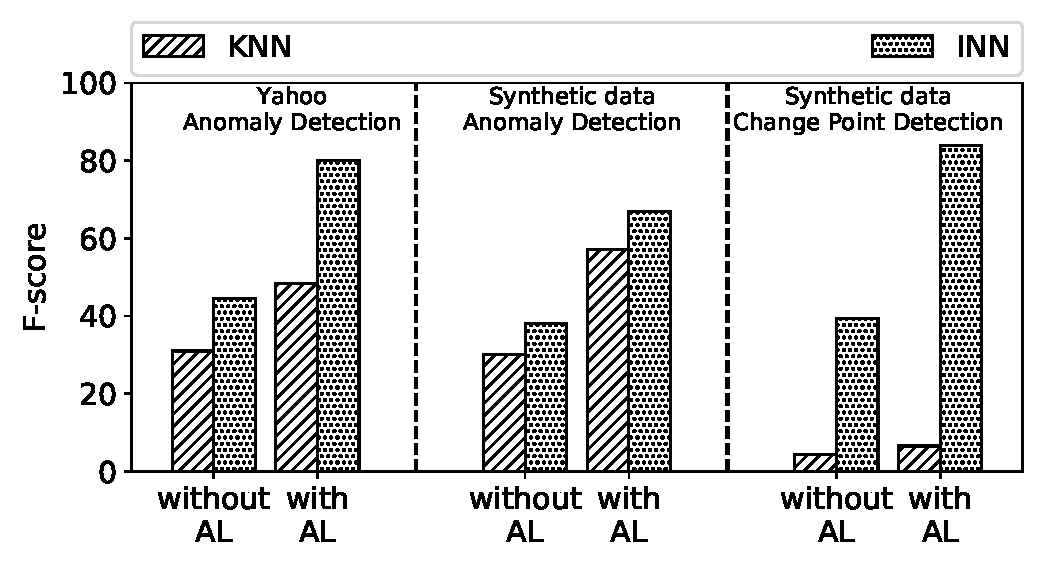
\includegraphics[width=0.8\textwidth]{Part3/Chapter7/figures/INNvsKNN_yahoo.pdf}
	\caption{ : Comparison the effectiveness of INN and KNN in two cases: before and after performing Active learning. From left to right, the two plots show: (a) Anomaly detection quality over Yahoo datasets, (b) Anomaly and change point detection quality over Synthetic datasets.}
	\label{fig:comapration_INNvsKNN_yahoo}
\end{figure}

The same results are found in the evaluation over synthetic datasets. CABD-INN outperforms CABD-KNN in all cases. Especially in change point detection, the f-score of CABD-INN achieves 39.3\% before AL and 83.8\% after AL respectively while that of CABD-KNN are only around 4.38\% and 6.55\%. These results prove again the superiority of INN over KNN. 

\subsection{Enhancing repairing quality}

To minimize the impact of anomalies on data reliability, a repairing process is usually triggered after anomaly detection. We evaluate the integration of our proposal with a recently proposed data-repairing algorithm, Iterative Minimum Repairing (IMR)~\cite{song2015screen,zhang2017time}. The experiment shows how the quality of the automatic data repairs of IMR improves by % randomly labeling 20\% data and 
labeling anomalies with the Active Learning mechanism of CABD. The repairing quality is presented by Root Mean Square (RMS) error that evaluates the distance between ground truth and repaired value. Lower RMS error values indicate better results. Figure~\ref{fig: IMR_optimization} illustrates the experiment over synthetic datasets with varying anomaly and change point percentages. IMR with CABD for the labelling of the data shows significantly better repairing results than the original IMR (based on random values selection) in all datasets. For example, in dataset ds-1 and ds-2, CABD reduces RMS error 4 times from about 74.5 and 85.4 to 16.7 and 18.9, respectively. Moreover, referring to Table~\ref{tab:gcz_data_synthetic}, with CABD, the average number of labelled points for synthetic datasets is 38.72. Given that there are 2000 data points, this means that CABD require the labeling of about 2\% data point to achieve such results. \\

In summary, these results prove the utility of our propose in both improving the repairing quality and in reducing the data labeling effort.

\subsection{Comparison of quality}
We do state-of-the-art a number of anomaly detection method but evaluating all of them is extremely heavy. The algorithms are evaluated including Numenta \cite{ahmad2017unsupervised}, KNN-CAD \cite{burnaev2016conformalized}, ContextOSE \cite{ContextOSE}, Multinomial Relative Entropy \cite{wang2011statistical}, Bayesian Online detection\cite{adams2007bayesian}. The NAB standard profile is used to determine abnormal points relied on anomaly score. The source code and parameter settings for all of the above algorithms are fetched from NAB repository. \\

A comparative analysis of detection quality on all datasets (Yahoo, IoT and Synthetic datasets) reported in Figure~\ref{fig:comapration_USVs_sync} shown that the detection quality presented by F-score of all reviewed algorithms is fairly low when dealing with various anomaly types. The average of F-measure is under 20\% even with the recent algorithms such as Numenta or KNN-CAD. That is, they may not deal with a large number of consecutive errors as well as the present of change points. Contrastingly, CABD always shows significantly better results on all cases (with and without applying active learning). The average F-measure scores before and after active learning on all datasets are about 45.3\% and 82\% respectively. \\

%This result demonstrates that our proposal works well in different anomaly types in wide-range scenarios.  

In a further study, we compare detection quality between CABD and the most common supervised outlier detection algorithms such as 
Angle-Based Outlier Detection (ABOD)~\cite{kriegel2008angle},
Clustering-Based Local Outlier Factor (CBLOF)~\cite{he2003discovering},
Feature Bagging (F-Bag)~\cite{lazarevic2005feature},
Isolation Forest (IF)~\cite{liu2008isolation},
Minimum Covariance Determinant (MCD)~\cite{hardin2004outlier},
Principal Component Analysis (PCA)~\cite{shyu2003novel},
Robust Covariance (R-CoV)~\cite{rousseeuw1999fast}, 
One-Class Support Vector Machines (SVM)~\cite{ma2003time}. 
These algorithms are trained by clean datasets which are eliminated abnormalities. In this evaluation, the source code of such algorithms are obtained from Python toolkit for detecting outlying objects~\cite{pyod}. Figure~\ref{fig:comapration_SVs_yahoo} presents the results on the Yahoo, IoT and synthetic datasets. Again, such results are similar to those in Figure~\ref{fig:comapration_USVs_sync}. That is, CABD always shows the significantly better performance comparing with others. For example, on Yahoo datasets, the average F-score of CABD after active learning is 80\% while the best of others is only 40\% (HBOS algorithm). Similarly, such scores on synthetic datasets are reported about 68\% and 38\% for CABD and best of supervised algorithms (Isolated Forest (IF) algorithm) respectively.

\begin{figure}[h]
	\centering
	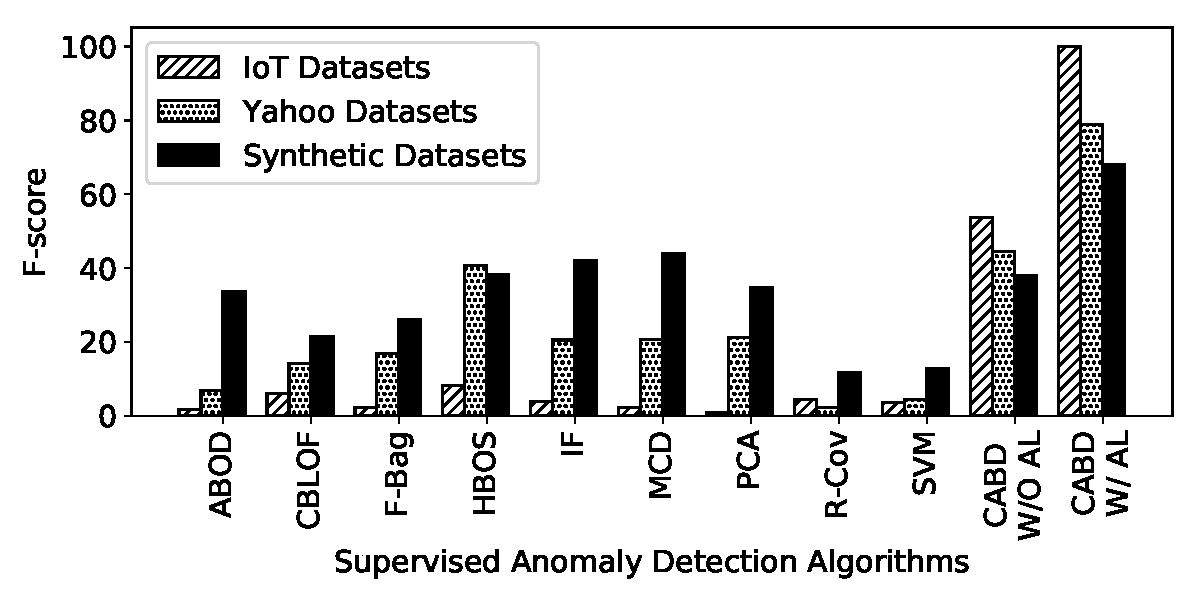
\includegraphics[width=0.8\textwidth]{Part3/Chapter7/figures/SVs_compare_yahoo_synthetic.pdf}
	\caption{ : Comparing detection quality with Supervised Anomaly Detection Algorithms over all datasets}
	\label{fig:comapration_SVs_yahoo}
\end{figure}

\begin{figure}[h]
	\centering
	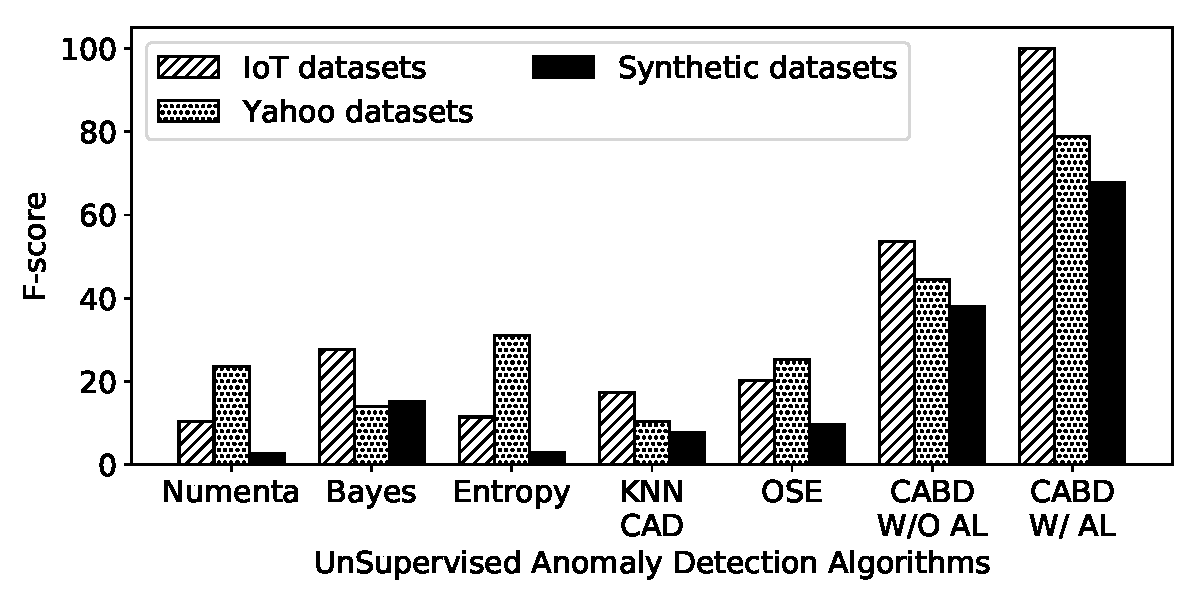
\includegraphics[width=0.8\textwidth]{Part3/Chapter7/figures/SVs_compare_unsuperviced_yahoo.pdf}
	\caption{ : Comparing detection quality with Unsupervised Anomaly Detection Algorithms over all datasets}
	\label{fig:comapration_USVs_sync}
\end{figure}

\section{Related Work}
The same ambition preserves the notable information from data cleaning process. The SCREEN algorithm~\cite{song2015screen}
works under the assumption that the speed of data changes (namely speed constraint) is constraint. This means the $jump$ of values is limited and considered as an anomaly if it is out of a given boundary. Based on such assumption, they propose a solution for stream data to identify and repair the  “jump” values in a given sequence (windows data) w.r.t the speed constraint while minimizing the repair distance. To achieve this goal, the authors introduce a novel concept named “Median Principle” to find the middle point of a specific sequence that is intuitively believed minimizing the repair distance. In addition, to deal with the trade off between choosing the window size and speed constraints. They proposed an adaptive windows size based recently extreme speed constraint (min or max speed). However, the SCREEN can show high performance in repairing single anomaly but hardly handle a collective anomaly. In addition, the repairing results strongly reply on the correctness of initial assumption. Being aware such limitations, a latter algorithm named Iterative Minimum Repairing (IMR)~\cite{zhang2017time} is proposed. The general idea of such algorithm is that combining between labeling some dirty observations and iterative repairing from high to low confidence repairs could enhance the performance. After each iteration, the parameter of the ARX~\cite{park2005outlier} model is calculated to generate the repair candidate list based on the difference of original and inferred data. The data point with minimum difference is repaired. The stop conditions of repairing procedure could be reaching the threshold of convergence or maximum number of iterations. The final goal of CABD, SCREEN and IRM is to preserve the notable information in time series data. But, we try to optimize the anomaly detection procedure while SCREEN and IRM aim to improve repairing procedure. Thus, they are not in our comparison base-line.  \\

In this section, we briefly review the concept of nearest neighbor analysis which has been used in the several contexts of anomaly detection. Such techniques detect the abnormality by examining the distance or similarity between two data instances. Normal data instances occur in dense neighborhoods, while anomalies occur far from their closet neighbors \cite{chandola2009anomaly}. The distance (or similarity) can be calculated in different way. For example: Euclidean distance is the wide usage for continuous attributes in \cite{Breunig:2000:LID:335191.335388}\cite{tang2001robust}\cite{kriegel2009loop}. For categorical attributes, a simple matching coefficient is often used but more complex distance measures can also be used \cite{boriah2008similarity}\cite{chandola2008understanding}. There are two main approaches in Nearest neighbor-based anomaly detection techniques: (1) Using the distance to the k nearest neighbor as anomaly score. (2) Computing the anomaly score from the relative density of each data point.\\

The original idea of nearest neighbor anomaly detection defines the anomaly score of a data instance as its distance to its $ k^{th} $ nearest neighbor in a given data set which is mentioned in \cite{byers1998nearest}. This work also has been applied to detect shorted turns in wind turbin-generators in \cite{guttormsson1999elliptical}. The basic technique is enhanced by researchers in various aspects. For example: The author in \cite{eskin2002geometric}\cite{angiulli2002fast}\cite{zhang2006detecting} calculates anomaly score from the sum of the distance to k nearest neighbors. \cite{knorr1997unified} counts the number of nearest neighbor within d distance as anomaly score. \cite{wu2006outlier} designs a simple sampling technique to reduces the complexity of algorithm. A Resolution Outlier Factor (ROF) was proposed in \cite{fan2006nonparametric}. According to this method, points are outliers or within a cluster depends on the resolution of applied distance thresholds. Conformalized density- and distance-based anomaly detection \cite{burnaev2016conformalized} measure the dissimilarity between observation by combining feature extraction method and conformal paradigm. This was shown to provide effective results for outlier analysis.\\

The density-based anomaly detection is based on the idea: “An instance that lies in a neighborhood with low density is declared to be anomalous while an instance that lies in a dense neighborhood is declared to be normal”. The most well-known algorithm in such technique is Local Outlier Factor (LOF)\cite{Breunig:2000:LID:335191.335388}. For given data instance, the anomaly score is basically the ratio of the average local densities of its k-nearest neighbors over the local density itself.  However, LOF ineffectively detects the regions which are not clearly separated. Several researches were subsequently proposed to extend the concept of LOF. The authors in \cite{jin2006ranking} uses symmetric nearest neighbor relationship to define the outlier score. \cite{tang2002enhancing} introduces a new variation of LOF named Connectivity-based Outlier Factor (COF)\cite{tang2001robust} which can detect the abnormality distributed on arbitrarily shaped clusters. The LOF is also combined with other techniques. For example, the work in \cite{he2002outlier}\cite{he2003discovering} calculate the anomaly score, named Cluster-Based Local Outlier Factor (CBLOF), from local distances to nearby cluster and the size of the clusters. The other method is LOCI, a truly density-based method, using the number of circular neighbors around data point as outlier score. Most of existing nearest neighbor anomaly detections are sensitive to define the k-nearest neighbors. \cite{ha2014robust} propose a new method using instability factor (INS) aiming to overcome the weakness relating the vulnerability of parameter configuration. The enhanced version of INS using “Natural Neighbor” concept is introduced in \cite{huang2016non}.
A more recent proposal is presented in \cite{wang2011statistical} using relative entropy as the distance measurement.\\

Additional algorithms for anomaly detection purpose on time serial data introduce in \cite{Lakhina:2004:DNT:1030194.1015492}\cite{1565683}. Twitter proposes an open-source method named Seasonal Hybrid ESD \cite{hochenbaum2017automatic} using seasonal decomposition and statistical metrics to correctly detect anomalies. Skyline \cite{skyline} and Loda \cite{Pevny2016} use an ensemble of various weak detections or statistical techniques to enhance the detection performance.The other method named KNN-CAD \cite{burnaev2016conformalized} uses a probabilistic model to interpret the distance based on the conformal paradigm. We include evaluation of these methods in our result section.
\par The key advantages of nearest neighbor-based method are unsupervised and independent with data distribution. This means they are purely data-driven \cite{chandola2009anomaly}. However, this method fall in two aspect: (1) it can not handle a sequence of continuous outliers or large collective anomalies due to be sensitive in parameter configuration. (2) It mis-detects the seasonal event as abnormality due to lacking frequency checking.  In contrast, our CABD approach, using new concept named invert nearest neighbor and applying active learning, could not only detect both single and collective anomalies with better accuracy but also highlight the valuable events. 

% \begin{figure}[h]
% 	\centering
% 	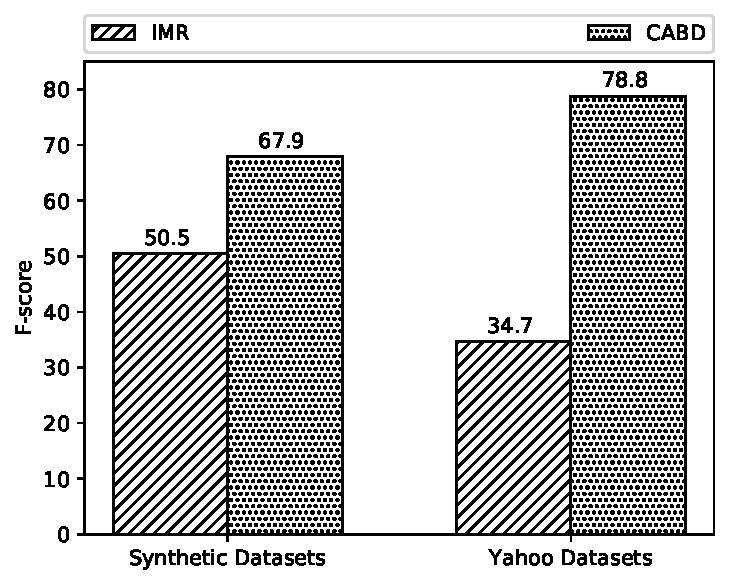
\includegraphics[width=0.4\textwidth]{CABDvsIMR.pdf}
% 	\caption{ : Comparing the anomaly detection quality between CABD and IMR over Yahoo and Synthetic datasets.}
% 	\label{fig:comapration_CABDvsIMR}
% \end{figure}



\section{Conclusion}

With the increase in connected devices in IoT, the anomaly detection is becoming increasingly important. We believe anomaly detection represents one of the most significant near-term applications for machine learning in IoT. In this work, we propose a new unsupervised algorithm for anomaly and breakpoint detection. The proposed method combines the novel concept named invert nearest neighbor and active learning. Unlike the most of previous outlier detection approached, our algorithm not only effectively detect s both single and collective anomaly but also preserves and highlights breakpoint. Moreover, we solve the challenge regarding the sensitiveness of parameters in existing methods by applying active learning to adapt the parameters. Experimental results clearly indicate that the effectiveness of the proposed method for real IoT user-cases. To further prove the effectiveness of invert nearest neighbor and active learning, we will apply them in not only anomaly detection but also clustering algorithms for future studies. 


